\section{External Transactions}
\label{section:external_transactions}

\begin{figure}[H]
\centering
\includegraphics[scale=0.48]{08_external_transactions/png/external_transactions}
\caption{External Transactions}
\label{fig:external_transactions}
\end{figure}

Figure \ref{fig:external_transactions} shows an external transaction. Without some extra form of
coordination, implemented by some additional accounts, the transaction as it stands in the figure
would be very difficult to coodinate. But it captures the important property of external
transactions, that across the market boundaries the exchange rate is the rate of payments in
currency $A$ as a ratio of the rate of payments in currency $B$.

\[
    X = \frac A  B
\]


where $X$ is the exchange rate and the unit is

\[
    \left[ \frac {\$} {yen} \right]
\]

Following our program, we'll look at how external transactions interact with other transaction
types.

\subsection{External Transactions and Exchange Transactions}

\begin{figure}[H]
\centering
\includegraphics[scale=0.48]{08_external_transactions/png/external_and_exchange_tx}
\caption{Interaction of External and Exchange Transactions}
\label{fig:external_and_exchange_tx}
\end{figure}

There is a negative feedback stabilizing process that brings the exchange rate into equilibrium with
the relative price levels of the two currencies. This process was described by Cassel
\cite{cassel1914} in 1914. If   

\[
    \frac {P_A} {P_B} > \frac A B
\]

the goods and services in currency $B$ are cheaper than goods and services in currency $A$, and so
exports of goods and services from $B$ to $A$ increase, and exports of goods and services from $A$
to $B$ decrease. This process continues until an equilibrium where

\[
    \frac {P_A} {P_B} \dot{=} \frac A B
\]

where $\dot{=}$ represents the equilibrium state.
